\section{PDC Overview}
\subsection*{History}

\frame{
\frametitle{History of PDC}

\footnotesize
\begin{table}
\begin{tabular}{r|r|r|r|l|l} \hline 
\textbf{Year} & \textbf{rank} & \textbf{procs.} & \textbf{peak TFlops} & \textbf{vendor} & \textbf{name} \\ \hline
2017 & 69  & 67456 & 2438.1 & Cray & Beskow\footnote{XC40 16-core 2.3GHz} \\ \hline
2014 & 32  & 53632 & 1973.7 & Cray & Beskow \\ \hline
2011 & 31  & 36384 & 305.63 & Cray & Lindgren\footnote{XE6 12-core 2.1 GHz} \\ \hline
2010 & 76  & 11016 & 92.534 & Cray & Lindgren \\ \hline
2010 & 89  & 9800  & 86.024 & Dell & Ekman\footnote{PowerEdge SC1435 Dual core Opteron 2.2GHz, Infiniband} \\ \hline
2005 & 65  & 886   & 5.6704 & Dell & Lenngren\footnote{PowerEdge 1850 3.2 GHz, Infiniband} \\ \hline
2003 & 196 & 180   & 0.6480 & HP & Lucidor\footnote{Cluster Platform 6000 rx2600 Itanium2 900 MHz Cluster, Myrinet} \\ \hline
1998 & 60  & 146   & 0.0934 & IBM & Strindberg\footnote{SP P2SC 160 MHz} \\ \hline
1996 & 64  & 96    & 0.0172 & IBM & Strindberg \\ \hline
1994 & 341 & 256   & 0.0025 & Thinking Machines & Bellman\footnote{CM-200/8k} \\ \hline
\end{tabular}
\end{table}
}

\subsection*{Member of SNIC}

\frame
{
\frametitle{SNIC}
\framesubtitle{Swedish National Infrastructure for Computing}
\begin{columns}
\column{.3\textwidth}

\includegraphics[width=0.7\linewidth]{snic.png}\\
%\vspace{-55mm}
\column{.7\textwidth}
\footnotesize
National \alert{research infrastructure} that provides a \alert{balanced and cost-efficient} set of \alert{resources and user support} for \alert{large scale computation and data storage} to meet the needs of researchers from all scientific disciplines and from all over Sweden (universities, university colleges, research institutes, etc).\\
\hfill \break
SNIC is funded by the Swedish Research Council (VR-RFI) and the 10 participating universities: Chalmers, GU, KI, KTH, LiU, LU, SLU, SU, UmU, and UU.
\end{columns}
}

\subsection*{Business}
\frame{
\frametitle{Collaboration with industry}
\begin{columns}
\column{.5\textwidth}
  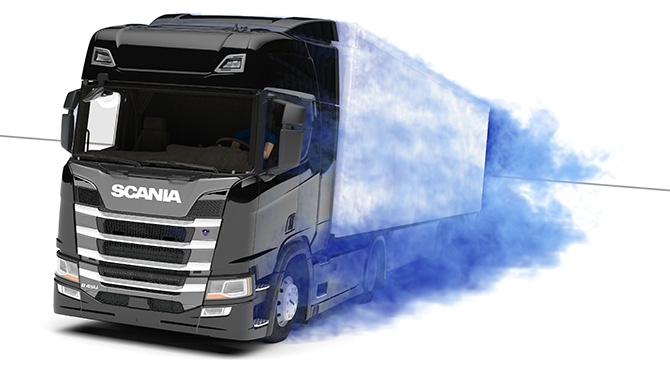
\includegraphics[width=\columnwidth]{Scania_truck}
\column{.5\textwidth}
\footnotesize
PDC's largest industrial partner is Scania. The figure shows a volume rendering of the instantaneous velocity magnitude on the leeward side of a Scania R20 Highline truck at crosswind conditions. (Source: Scania)
\end{columns}
\begin{itemize}
    \footnotesize
    \item Business partners \\
        \scriptsize
        \href{https://www.pdc.kth.se/research/business-research/pdc-partners}{https://www.pdc.kth.se/research/business-research/pdc-partners}
    \footnotesize
    \item White papers from research collaborations between PDC and European companies \\
        \scriptsize
        \href{https://www.pdc.kth.se/research/business-research/white-papers-1.737818}{https://www.pdc.kth.se/research/business-research/white-papers-1.737818}
    \footnotesize
    \item A small part of Dardel nodes will be dedicated to industry/business research.
    \item If you are interested in purchasing HPC compute time, contact PDC Support.
\end{itemize}
}

\subsection*{Training}
\frame{
  \frametitle{Broad Range of Training}
  \begin{description}
  \item [Summer School]
    Introduction to HPC held every year
  \item [Courses]
    \begin{itemize}
    %\item Programming for GPU
    \item Distributed and Parallel Computing
    \item Cloud Computing
    \item Programming for GPU
    \item Software Development Tools
    %\item CodeRefinery workshops
    \end{itemize}
  \item [PDC User Days] PDC Pub and Open House
  \end{description}
  \begin{columns}
    \column{.3\textwidth}
    \includegraphics[width=0.9\linewidth]{class3}
    \column{.3\textwidth}
    \includegraphics[width=0.9\linewidth]{class2}
    \column{.3\textwidth}
    \includegraphics[width=0.9\linewidth]{class1}
  \end{columns}
}

\subsection*{Staff}
\frame{
\frametitle{Support and System Staff}
\begin{exampleblock}{First-line support}
  Provide specific assistance to PDC users related to accounts, login, allocations etc.
\end{exampleblock}
\begin{exampleblock}{System staff}
  System managers/administrators ensure that computing and storage resources run smoothly and securely.
\end{exampleblock}
\begin{exampleblock}{Application Experts}
  Hold PhD degrees in various fields and specialize in HPC. Assist researchers in optimizing, scaling and enhancing scientific codes for current and next generation supercomputers.
\end{exampleblock}
}
